\chapter{Risultati sperimentali}
\label{chap:risultati}
\vspace{1cm}
Questo capitolo illustra i risultati del lavoro, descrivendo
il procedimento effettuato per validare la metodologia proposta
in questa tesi.

La sezione \ref{sec:ambienteTest} descrive l'ambiente e le
modalit\`a con cui sono stati ricavati i risultati contenuti
in questo capitolo.

La sezione \ref{sec:risultatiEsplorazione} mostra i grafici relativi
ai risultati ottenuti eseguendo l'algoritmo di esplorazione.

\newpage

\section{Ambiente di test}
\label{sec:ambienteTest}

La metodologia proposta \`e stata valutata mediante l'esecuzione
dell'algoritmo di esplorazione su un insieme di task graph,
con diverse architetture di riferimento.

I task graph usati come benchmark per la validazione del funzionamento di
MapR sono stati generati utilizzando \ac{TGFF} \cite{tgff}, uno strumento per
la generazione di task graph pseudo-casuali ampiamente utilizzato.
I task graph cos\`i generati differiscono nel numero di nodi (task) e di implementazioni
disponibili per ciascun task. Ogni implementazione \`e caratterizzata dai propri requisiti
di area e tempo di esecuzione. Per effettuare i test sui benchmark \`e stato generato un insieme di 25 task graph da
10, 20, 30, 40, 50 nodi (5 istanze per ogni numero di nodi).

\begin{figure}[t]
  \begin{center}
    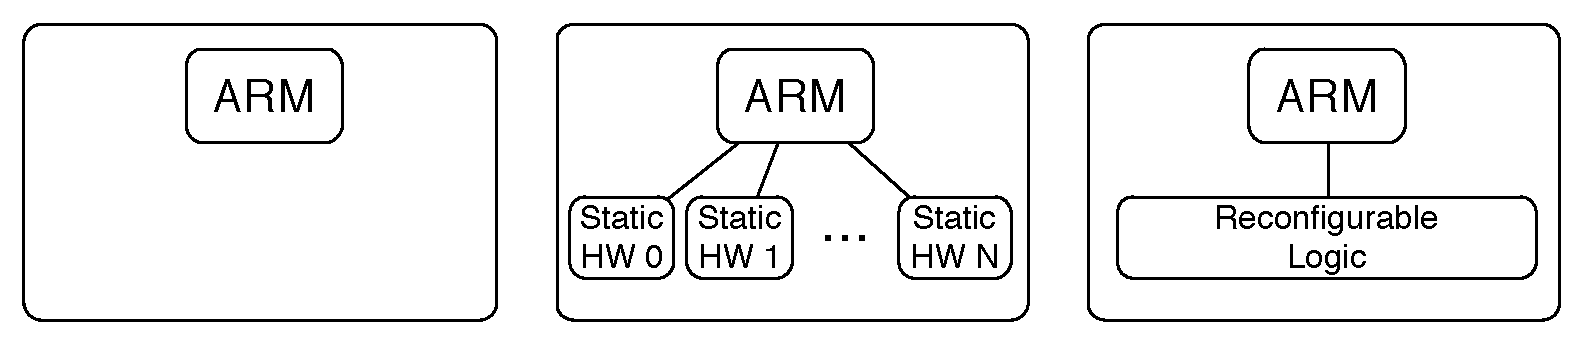
\includegraphics[width=0.7\textwidth]{./capitoli/figure/cap6/templates.pdf}
    \caption{Architetture di riferimento utilizzate per i test su benchmark sintetici.}
    \label{fig:architettureTestSintetici}
  \end{center}
\end{figure}

Le architetture utilizzate
sono rappresentate in figura \ref{fig:architettureTestSintetici}. La prima \`e un'architettura puramente
software che serve da baseline; in questo caso il tool non pu\`o utilizzare risorse hardware.
La seconda \`e caratterizzata anche da processing element hardware \emph{statici}, quindi MapR non pu\`o
sfruttare le potenzialit\`a della riconfigurazione, tuttavia \`e possibile mappare task in hardware.
L'ultima architettura \`e caratterizzata dalla presenza di una o pi\`u aree riconfigurabili, in questo
caso la riconfigurazione parziale dinamica pu\`o essere sfruttata da MapR.
% TODO descrivere il numero di core delle architetture utilizzate


\section{Risultati dell'esplorazione}
\label{sec:risultatiEsplorazione}
Dopo aver generato i task graph con le modalit\`a descritte nella precedente
sezione, l'esplorazione \`e stata eseguita e i makespan relativi alla migliore soluzione
trovata nell'esplorazione corrente sono stati salvati per tutte le architetture.
La funzione obiettivo dell'algoritmo di esplorazione utilizzata per questi esperimenti
\`e basata solamente sulla stima del makespan calcolata dallo scheduler descritta nel
capitolo \ref{chap:approccio}.
% TODO descrivere i parametri di task graph for free utilizzati

\begin{figure}[t]
 \begin{center}
  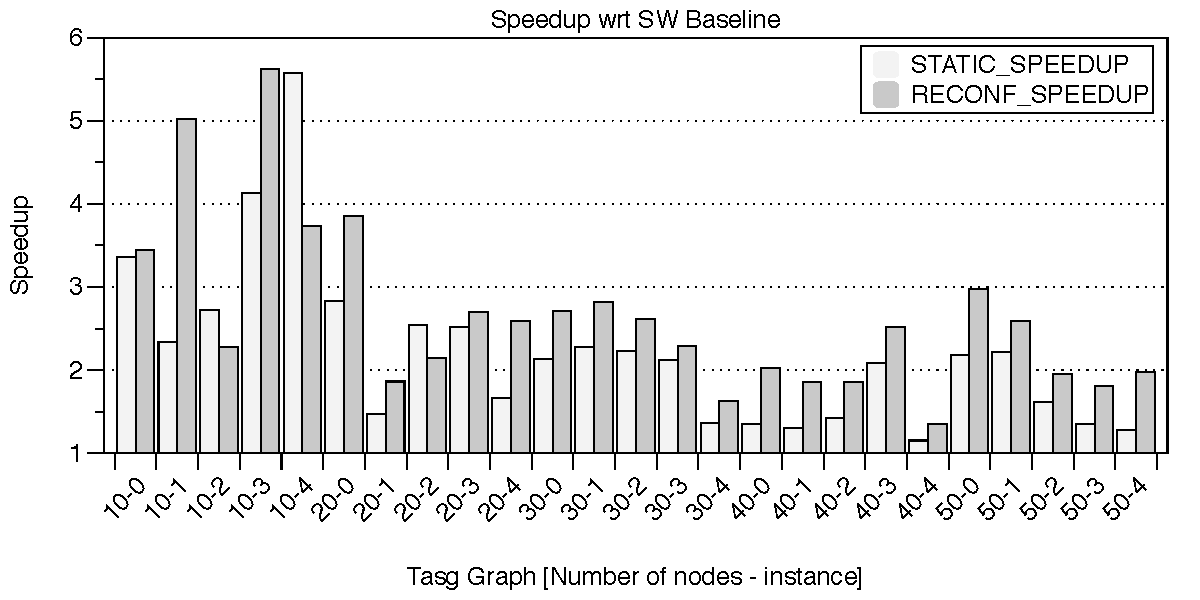
\includegraphics[width=\textwidth]{./capitoli/figure/cap6/FPL_makespan.pdf}
  \caption{Speedup dell'architettura statica e riconfigurabile rispetto alla
  baseline software.}
  \label{fig:speedupBaseline}
 \end{center}
\end{figure}

\subsubsection{Speedup rispetto a baseline software}
La figura \ref{fig:speedupBaseline} rappresenta lo speedup ottenuto utilizzando
le architetture hardware statica e riconfigurabile rispetto alla baseline
con implementazioni esclusivamente software, per tutti i task graph oggetto
dell'esplorazione. Si pu\`o vedere che per tutti i task graph MapR riesce ad
avere uno speedup rispetto alla baseline, che varia da circa $2\text{x}$ per istanze con
un elevato numero di nodi, fino a $5,5\text{x}$ con istanze pi\`u piccole. La differenza
tra gli speedup rappresentati in figura \ref{fig:speedupBaseline} \`e dovuta al fatto che,
pur avendo lo stesso numero di nodi, le istanze in realt\`a hanno topologie e tempi di
esecuzione potenzialmente molto diversi: questo fattore influisce sulla lunghezza dello schedule
al termine dell'esplorazione.
Inoltre, si pu\`o vedere dalla figura che, con il crescere della dimensione dei task graph e
conseguente scarsit\`a di risorse hardware, MapR riesce a sfruttare efficacemente la riconfigurazione
parziale dinamica e a ottenere risultati migliori impiegando l'architettura riconfigurabile.

\begin{figure}[t]
 \begin{center}
  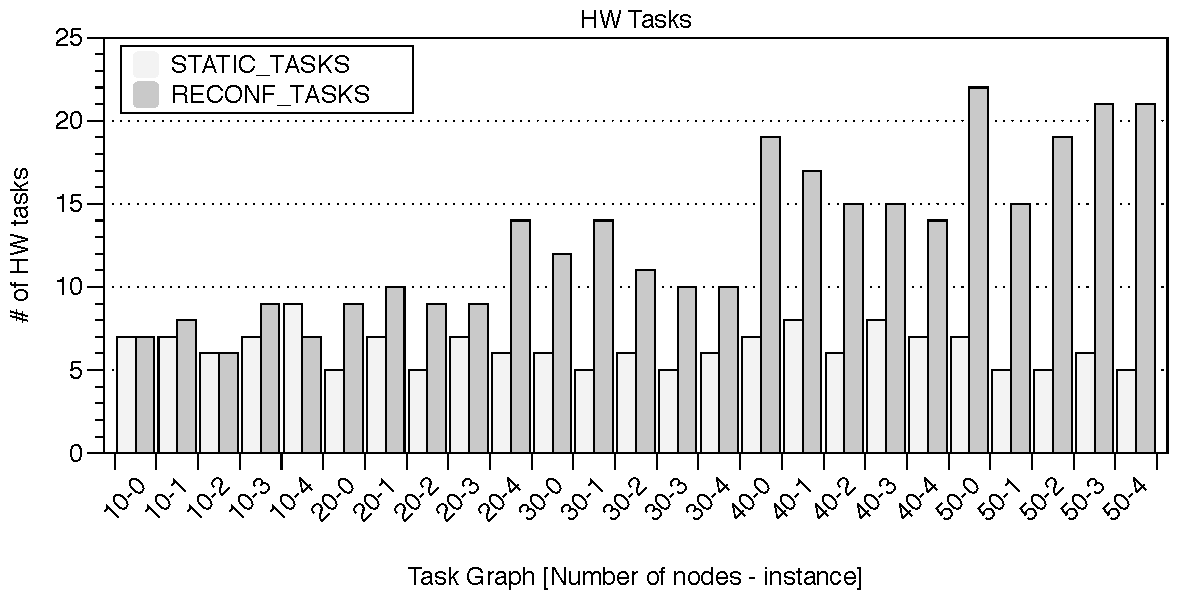
\includegraphics[width=\textwidth]{./capitoli/figure/cap6/FPL_HWtasks.pdf}
  \caption[Numero di task implementati in hardware.]{Numero di task implementati in hardware; dati relativi ai due template architetturali
  che possono utilizzare la logica riconfigurabile.}
  \label{fig:hardwareTask}
 \end{center}
\end{figure}

\subsubsection{Mapping dei task}
La figura \ref{fig:hardwareTask} rappresenta il numero di task che sono stati mappati
dall'algoritmo di esplorazione su logica riconfigurabile.
In questo caso sono stati considerati i due template architetturali che permettono
l'utilizzo della logica riconfigurabile, dando piena libert\`a
a MapR di decidere quanti e quali task mappare su core statici o regioni riconfigurabili del dispositivo.
I risultati confermano quanto anticipato nel paragrafo precedente: al crescere del numero di
task quando le risorse hardware sono scarse, in ottica di minimizzazione del makespan, la possibilit\`a di sfruttare
la riconfigurazione parziale permette a MapR di spostare
in hardware un maggior numero di task, sfruttando meglio l'area a disposizione; 

Ad esempio, considerando l'ultimo task graph (50-4), MapR \`e riuscito ad ottenere uno speedup di
$1,2\text{x}$ nel caso statico implementando 5 task in hardware; avendo a disposizione l'architettura
riconfigurabile, lo speedup ottenuto \`e stato di $2\text{x}$ rispetto alla baseline software,
spostando 21 task in hardware.


\begin{figure}[t]
 \begin{center}
  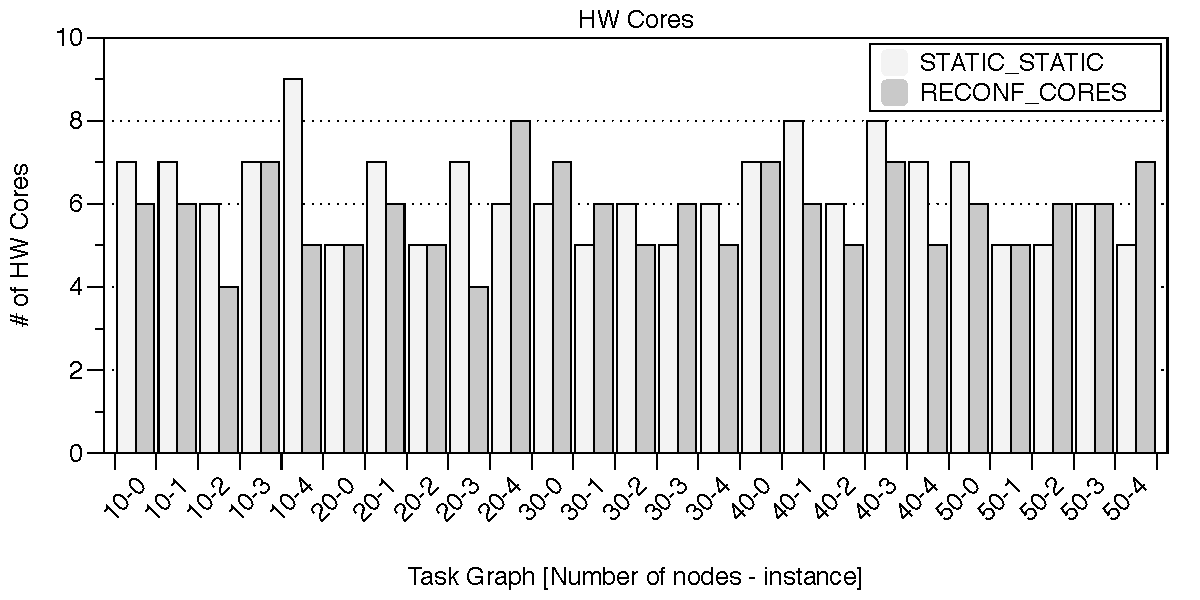
\includegraphics[width=\textwidth]{./capitoli/figure/cap6/FPL_HWcores.pdf}
  \caption{Numero di core utilizzati con architettura statica e riconfigurabile.}
  \label{fig:coreUtilizzati}
 \end{center}
\end{figure}



\begin{figure}[t]
 \begin{center}
  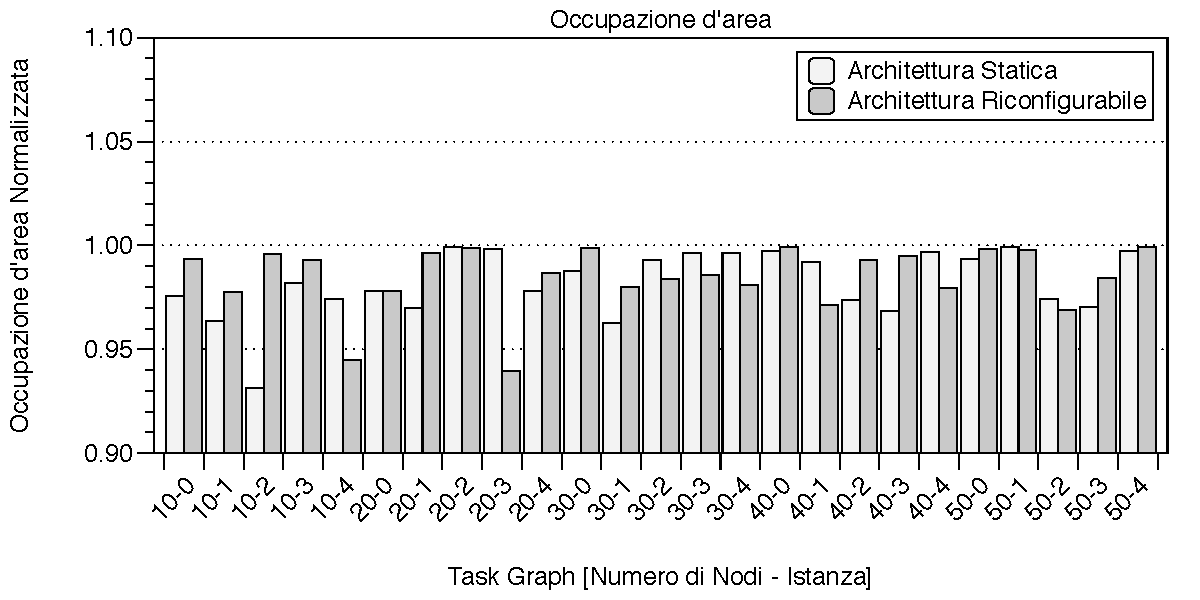
\includegraphics[width=\textwidth]{./capitoli/figure/cap6/FPL_Area.pdf}
  \caption{Uso dell'area, normalizzato rispetto all'area totale.}
  \label{fig:usoArea}
 \end{center}
\end{figure}



\begin{figure}[t]
 \begin{center}
  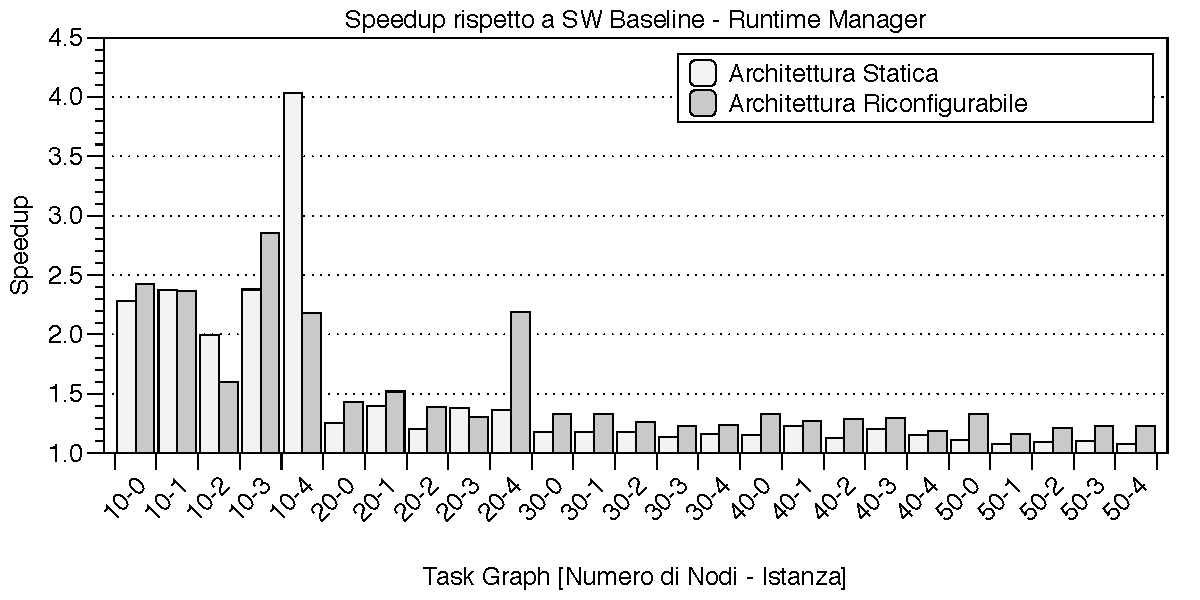
\includegraphics[width=\textwidth]{./capitoli/figure/cap6/FPL_Runtime.pdf}
  \caption{Speedup dell'architettura statica e riconfigurabile rispetto alla
  baseline software, dopo l'esecuzione sul dispositivo.}
  \label{fig:speedupBaselineRuntime}
 \end{center}
\end{figure}
